% Original teaching adaptation of Heather Macbeth, The Mechanics of Proof, Chapter 8.
% Source: https://hrmacbeth.github.io/math2001/08_Functions.html
% Source repository: hrmacbeth/math2001, e660f42b13ddcb6d12b52ba036d6bd071a0cfb9b.
% Mathematical statements and examples are attributed below; prose and TikZ drawings are new.
% Lean listings are ASCII teaching demonstrations in the book's environment, not build-verified.
% CSC302 lecture slides adapted from Heather Macbeth, The Mechanics of Proof.
\documentclass[aspectratio=169,11pt]{beamer}
\usepackage[T1]{fontenc}
\usepackage{lmodern}
\usepackage{amsmath,amssymb,mathtools}
\usepackage{booktabs,array,listings,tikz}
\usetikzlibrary{arrows.meta,positioning,calc}
\definecolor{ProofNavy}{HTML}{18324F}
\definecolor{ProofTeal}{HTML}{007D82}
\definecolor{ProofPaper}{HTML}{F3F6F8}
\usetheme{default}
\setbeamercolor{normal text}{fg=ProofNavy,bg=white}
\setbeamercolor{structure}{fg=ProofTeal}
\setbeamercolor{frametitle}{fg=ProofNavy}
\setbeamercolor{block title}{fg=white,bg=ProofNavy}
\setbeamercolor{block body}{fg=ProofNavy,bg=ProofPaper}
\setbeamercolor{block title example}{fg=white,bg=ProofTeal}
\setbeamercolor{block body example}{fg=ProofNavy,bg=ProofPaper}
\setbeamerfont{frametitle}{size=\Large,series=\bfseries}
\setbeamertemplate{navigation symbols}{}
\setbeamertemplate{itemize item}{\small\textbullet}
\setbeamertemplate{footline}{%
  \leavevmode\hbox{%
  \begin{beamercolorbox}[wd=.86\paperwidth,ht=2.8ex,dp=1.2ex,leftskip=1.6em]{author in head/foot}%
    \scriptsize CSC302\quad\textbar\quad\insertshorttitle
  \end{beamercolorbox}%
  \begin{beamercolorbox}[wd=.14\paperwidth,ht=2.8ex,dp=1.2ex,rightskip=1.6em plus1fil]{date in head/foot}%
    \scriptsize\insertframenumber/\inserttotalframenumber
  \end{beamercolorbox}}}
\setbeamersize{text margin left=8mm,text margin right=8mm}
\lstdefinelanguage{Lean}{%
  morekeywords={example,theorem,lemma,def,by,calc,have,exact,apply,intro,intros,constructor,rcases,rfl,rw,ring,numbers,linarith,nlinarith,rel,extra,addarith,obtain,left,right,use,choose,dsimp,change,ext,fun,show,from,at,with,induction,case,decide,contradiction,push_neg,by_cases,by_contra,assumption,existsi,simp,simpa},
  sensitive=true,morecomment=[l]{--},morestring=[b]"}
\lstset{language=Lean,basicstyle=\ttfamily\small,keywordstyle=\color{ProofTeal}\bfseries,
  commentstyle=\color{gray},stringstyle=\color{ProofNavy},showstringspaces=false,
  columns=fullflexible,keepspaces=true,breaklines=true,frame=single,
  rulecolor=\color{ProofTeal!30},backgroundcolor=\color{ProofPaper},
  aboveskip=0.5em,belowskip=0.4em}
\newcommand{\N}{\mathbb{N}}
\newcommand{\Z}{\mathbb{Z}}
\newcommand{\Q}{\mathbb{Q}}
\newcommand{\R}{\mathbb{R}}
\newcommand{\coursechapter}[2]{%
  \title[Chapter #1: #2]{Chapter #1\\#2}%
  \subtitle{The Mechanics of Proof \textbar{} CSC302 lecture notes}%
  \author{Based on Heather Macbeth's textbook}%
  \date{}%
}
\newcommand{\sourcecredit}[1]{\par\vfill{\tiny Source: Heather Macbeth, \emph{The Mechanics of Proof}, #1.}}
\newcommand{\bookurl}{\url{https://hrmacbeth.github.io/math2001/}}
\hypersetup{colorlinks=true,urlcolor=ProofTeal,linkcolor=ProofNavy}

\coursechapter{8}{Functions}
\begin{document}
\begin{frame}
  \titlepage
\end{frame}

% Source: Chapter 8 introduction and Example 8.1.1.
\begin{frame}{What we will learn}
\begin{itemize}
  \item Read a function's \emph{domain}, \emph{codomain}, and rule together.
  \item Prove or refute injectivity, surjectivity, and bijectivity.
  \item Use composition and inverses to organize proofs.
  \item Work with ordered pairs and a bijection $\N^2\to\N$.
\end{itemize}
\begin{block}{A function includes its types}
$f:X\to Y$ assigns exactly one element $f(x)\in Y$ to every $x\in X$.
Its \emph{image} is the set of outputs actually attained; its codomain is all of $Y$.
\end{block}
The rules $n\mapsto 2n$ on $\Z$ and $x\mapsto 2x$ on $\R$ have different surjectivity behavior.
\sourcecredit{Section 8.1}
\end{frame}

\section{8.1 Injectivity and surjectivity}
% Source: Definition 8.1.2 and finite-function Examples 8.1.8--8.1.11.
% The finite labels and diagram here are original.
\begin{frame}{8.1: Injectivity asks whether outputs identify inputs}
\begin{block}{Definition}
$f:X\to Y$ is \emph{injective} when
\[
  \forall x_1,x_2\in X,\qquad f(x_1)=f(x_2)\ \Longrightarrow\ x_1=x_2.
\]
\end{block}
\begin{columns}[T]
\begin{column}{.49\textwidth}
\centering
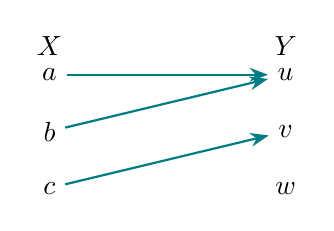
\begin{tikzpicture}[x=1cm,y=.72cm,>=Stealth]
\node at (0,2.5) {$X$}; \node at (3,2.5) {$Y$};
\foreach \label/\height in {a/2,b/1,c/0}{\node (x\label) at (0,\height) {$\label$};}
\foreach \label/\height in {u/2,v/1,w/0}{\node (y\label) at (3,\height) {$\label$};}
\draw[->,thick,ProofTeal] (xa)--(yu);
\draw[->,thick,ProofTeal] (xb)--(yu);
\draw[->,thick,ProofTeal] (xc)--(yv);
\end{tikzpicture}
\end{column}
\begin{column}{.48\textwidth}
This function is not injective: $a\ne b$ but $f(a)=f(b)=u$.
\medskip

A counterexample must give \emph{two distinct inputs with the same output}.
An unused output concerns surjectivity instead.
\end{column}
\end{columns}
\sourcecredit{Definition 8.1.2; Examples 8.1.8--8.1.11}
\end{frame}

% Source: Examples 8.1.1, 8.1.3, 8.1.4.
% Correction: Example 8.1.3's prose changes +3 to +1; preserve q(x)=x+3 throughout.
\begin{frame}{Two complete injectivity arguments}
\begin{exampleblock}{Translation: $q:\R\to\R$, $q(x)=x+3$}
Let $x_1,x_2\in\R$ and assume $q(x_1)=q(x_2)$. Then
\[
 x_1+3=x_2+3\quad\Longrightarrow\quad x_1=x_2
\]
by subtracting $3$. These inputs were arbitrary, so $q$ is injective.
\end{exampleblock}
\begin{exampleblock}{Squaring: $s:\R\to\R$, $s(x)=x^2$}
Choose $x_1=-1$ and $x_2=1$. We have
\[
 s(-1)=1=s(1),\qquad -1\ne 1.
\]
Thus $s$ fails the defining implication and is not injective.
\end{exampleblock}
\sourcecredit{Examples 8.1.3--8.1.4}
\end{frame}

% Source: Definition 8.1.5 and Examples 8.1.6--8.1.7.
\begin{frame}{Surjectivity asks whether every target is reached}
\begin{block}{Definition}
$f:X\to Y$ is \emph{surjective} when
$\forall y\in Y,\ \exists x\in X,\ f(x)=y$.
\end{block}
\textbf{Example.} Let $f:\Q\to\Q$ satisfy $f(x)=3x+2$.
Given any $y\in\Q$, choose $x=(y-2)/3\in\Q$. Then
\[
 f(x)=3\frac{y-2}{3}+2=y.
\]
The witness depends on the arbitrary target $y$, so this proves surjectivity.
\medskip

\textbf{Failure.} Squaring $\R\to\R$ misses $-1$, since $x^2\ge0$ for every real $x$.
A failed search for a witness is insufficient; we proved no witness can exist.
\sourcecredit{Definition 8.1.5; Examples 8.1.6--8.1.7}
\end{frame}

% Source: Lean demonstrations in Examples 8.1.3 and 8.1.6.
% ASCII spellings and anonymous functions replace the book's named functions.
\begin{frame}[fragile]{From quantifiers to Lean proof steps}
\begin{lstlisting}
example : Function.Injective
    (fun x : Real => x + 3) := by
  intro x1 x2 h
  dsimp at h
  addarith [h]

example : Function.Surjective
    (fun x : Rat => 3 * x + 2) := by
  intro y
  use (y - 2) / 3
  dsimp
  ring
\end{lstlisting}
\texttt{intro} selects arbitrary inputs or a target; \texttt{use} supplies a preimage.
For negative claims, unfold the property and use \texttt{push\_neg}.
\sourcecredit{Examples 8.1.3 and 8.1.6; illustrative textbook-environment code}
\end{frame}

% Source: Exercises 8.1.13, doubling on R versus Z; finite-table task is original.
\begin{frame}{Practice 8.1: Give a proof or a specific obstruction}
\begin{enumerate}
\item Is $x\mapsto2x$ surjective as a function $\R\to\R$? As a function $\Z\to\Z$?
\item Let $X=\{a,b,c\}$ and $Y=\{u,v\}$, with
\[
\begin{array}{c|ccc}
x&a&b&c\\\hline
f(x)&u&v&u
\end{array}
\]
Is $f:X\to Y$ injective? Is it surjective?
\end{enumerate}
For each positive answer, account for every relevant input or target.
For each negative answer, state the exact witnesses.
\sourcecredit{Exercises 8.1.13; original finite-table exercise}
\end{frame}

% Source: Solutions newly written for the preceding adapted/original exercises.
\begin{frame}{Practice 8.1: Solution ideas}
\begin{enumerate}
\item Over $\R$, target $y$ has preimage $y/2$, because $2(y/2)=y$.
Over $\Z$, target $1$ has no preimage: $2n$ is even for every $n\in\Z$.
\item The finite function is not injective: $a\ne c$ and $f(a)=f(c)=u$.
It is surjective: $u$ has preimage $a$, and $v$ has preimage $b$.
These are all the targets in $Y$.
\end{enumerate}
\begin{block}{Proof structure in Lean}
Surjectivity over a finite type: \texttt{intro y}, then \texttt{cases y}, then a witness in each case.
The book's \texttt{exhaust} handles the resulting concrete finite statements.
\end{block}
\sourcecredit{Examples 8.1.9 and 8.1.11; Exercises 8.1.13}
\end{frame}

\section{8.2 Bijectivity}
% Source: Definition 8.2.1 and Example 8.2.2.
\begin{frame}{8.2: Bijectivity combines two obligations}
\begin{block}{Definition}
$f:X\to Y$ is \emph{bijective} when it is both injective and surjective.
\end{block}
\textbf{Example.} Let $p:\R\to\R$, $p(x)=2x-5$.
\begin{enumerate}
\item \textbf{Injectivity.} If $p(x_1)=p(x_2)$, then
$2x_1-5=2x_2-5$. Adding $5$ and dividing by $2$ gives $x_1=x_2$.
\item \textbf{Surjectivity.} Given $y\in\R$, let $x=(y+5)/2$. Then
\[
p(x)=2\frac{y+5}{2}-5=y.
\]
\end{enumerate}
Both parts hold with domain and codomain $\R$, so $p$ is bijective.
\sourcecredit{Definition 8.2.1; Example 8.2.2}
\end{frame}

% Source: Theorem in Example 8.2.5; original compressed proof organization.
\begin{frame}{A bijection gives exactly one preimage}
\begin{block}{Theorem}
For $f:X\to Y$, $f$ is bijective if and only if
\[
 \forall y\in Y,\quad \exists!x\in X\text{ such that }f(x)=y.
\]
\end{block}
\textbf{Forward.} Surjectivity gives a preimage $x$ of $y$. If $f(x')=y$ also,
then $f(x')=f(x)$; injectivity gives $x'=x$.
\medskip

\textbf{Backward.} Existence gives surjectivity. To prove injectivity, assume
$f(x_1)=f(x_2)$ and call their common output $y$. Both $x_1$ and $x_2$ are preimages
of $y$, so uniqueness gives $x_1=x_2$.
\sourcecredit{Example 8.2.5}
\end{frame}

% Source: Example 8.2.2, same mathematics with the book's addarith tactic.
\begin{frame}[fragile]{Lean: Split the bijection proof}
\begin{lstlisting}
example : Function.Bijective
    (fun x : Real => 2 * x - 5) := by
  constructor
  case left =>
    intro x1 x2 h
    dsimp at h
    addarith [h]
  case right =>
    intro y
    use (y + 5) / 2
    dsimp
    ring
\end{lstlisting}
\texttt{constructor} separates injectivity from surjectivity.
To refute bijectivity, it is enough to refute either part.
\sourcecredit{Examples 8.2.2--8.2.4; illustrative textbook-environment code}
\end{frame}

% Source: Example 8.2.7 and Exercises 8.2.8.
\begin{frame}{Practice 8.2: Two ways a bijection can fail}
\begin{enumerate}
\item For $s:\N\to\N$, $s(n)=n+1$, prove injectivity and disprove bijectivity.
\item For $h:\R\to\R$, $h(x)=x^2+2x$, disprove bijectivity using two inputs.
\end{enumerate}
\begin{block}{Plan before calculating}
For the first function, look for a target below every output.
For the second, factor $x^2+2x=x(x+2)$ and compare its zeros.
\end{block}
\sourcecredit{Example 8.2.7; Exercises 8.2.8}
\end{frame}

% Source: Newly written solutions for Example 8.2.7 and Exercises 8.2.8.
\begin{frame}{Practice 8.2: Solution ideas}
\begin{enumerate}
\item If $n_1+1=n_2+1$, cancellation gives $n_1=n_2$, so $s$ is injective.
But $s(n)=n+1>0$ for all $n\in\N$. Thus $0$ has no preimage, and $s$ is not bijective.
\item We have $h(0)=0$ and $h(-2)=4-4=0$, whereas $0\ne-2$.
Thus $h$ is not injective, which already disproves bijectivity.
\end{enumerate}
\begin{block}{Finite versus infinite domains}
On the same finite type, an injective self-map is bijective (the book checks small examples).
The successor function shows that the analogous statement for $\N$ is false.
\end{block}
\sourcecredit{Examples 8.2.6--8.2.7; Exercises 8.2.8}
\end{frame}

\section{8.3 Composition of functions}
% Source: Definitions 8.3.1 and 8.3.3, Example 8.3.2.
\begin{frame}{8.3: Composition follows the types}
\begin{center}
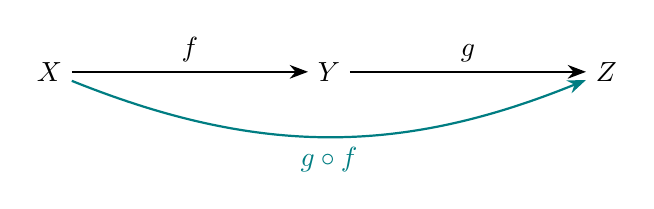
\begin{tikzpicture}[>=Stealth,node distance=30mm]
\node (X) {$X$}; \node[right=of X] (Y) {$Y$}; \node[right=of Y] (Z) {$Z$};
\draw[->,thick] (X)--node[above] {$f$}(Y);
\draw[->,thick] (Y)--node[above] {$g$}(Z);
\draw[->,ProofTeal,thick] (X) to[bend right=22] node[below] {$g\circ f$}(Z);
\end{tikzpicture}
\end{center}
For $f:X\to Y$ and $g:Y\to Z$, define $(g\circ f)(x)=g(f(x))$.
The identity $\operatorname{id}_X:X\to X$ satisfies $\operatorname{id}_X(x)=x$.
\medskip

If $f(x)=x+3$ and $g(x)=2x$ on $\R$, then
\[
 (g\circ f)(x)=2(x+3)=2x+6,
 \qquad (f\circ g)(x)=2x+3.
\]
Order matters. Equality of functions means equality at \emph{every} input.
\sourcecredit{Definitions 8.3.1 and 8.3.3; Example 8.3.2}
\end{frame}

% Source: Example 8.3.2; composition is expanded to an ASCII anonymous function.
\begin{frame}[fragile]{Lean: Extensionality changes the kind of goal}
\begin{lstlisting}
def f (x : Real) : Real := x + 3
def g (x : Real) : Real := 2 * x
def h (x : Real) : Real := 2 * x + 6

example : (fun x => g (f x)) = h := by
  ext x
  dsimp [f, g, h]
  ring
\end{lstlisting}
\begin{center}
\begin{tabular}{ll}
\toprule
Before \texttt{ext x} & Equality of two functions\\
After \texttt{ext x} & Equality of their values at an arbitrary $x$\\
After \texttt{dsimp} & $2(x+3)=2x+6$\\
\bottomrule
\end{tabular}
\end{center}
\sourcecredit{Example 8.3.2; illustrative textbook-environment code}
\end{frame}

% Source: Definition 8.3.5 and Example 8.3.4.
\begin{frame}{An inverse must undo the function in both directions}
\begin{block}{Definition}
For $f:X\to Y$, a function $g:Y\to X$ is an \emph{inverse} if
\[
 g\circ f=\operatorname{id}_X
 \qquad\text{and}\qquad
 f\circ g=\operatorname{id}_Y.
\]
Equivalently: $g(f(x))=x$ for every $x\in X$, and $f(g(y))=y$ for every $y\in Y$.
\end{block}
For $s:\R\to\R$, $s(x)=5-x$, we obtain
\[
 s(s(x))=5-(5-x)=x\qquad(x\in\R).
\]
Thus $s$ is its own inverse. Since the two functions are the same here,
the one calculation establishes both required identities.
\sourcecredit{Definition 8.3.5; Example 8.3.4}
\end{frame}

% Source: Propositions 8.3.7--8.3.8 and Theorem 8.3.9.
\begin{frame}{A function is bijective exactly when it has an inverse}
\textbf{Suppose $f:X\to Y$ is bijective.}
For each $y$, let $g(y)$ be its unique preimage. Then $f(g(y))=y$.
For any $x$,
\[
 f(g(f(x)))=f(x)\quad\Longrightarrow\quad g(f(x))=x
\]
by injectivity. Hence $g$ is an inverse.
\medskip

\textbf{Suppose $g:Y\to X$ is an inverse.}
If $f(x_1)=f(x_2)$, then
\[
x_1=g(f(x_1))=g(f(x_2))=x_2.
\]
For any $y\in Y$, $g(y)\in X$ is a preimage because $f(g(y))=y$.
Thus $f$ is injective and surjective.
\sourcecredit{Examples 8.3.7--8.3.9; Lean uses \texttt{choose} to select preimages}
\end{frame}

% Source: Exercises 8.3.10, inverse of 5x+1 and composition preservation.
\begin{frame}{Practice 8.3: Build a function proof from smaller ones}
\begin{enumerate}
\item Let $u:\R\to\R$ satisfy $u(x)=5x+1$. Find an inverse and verify both compositions.
\item Let $f:X\to Y$ and $g:Y\to Z$ be injective. Prove $g\circ f$ is injective.
\item With the same types, assume instead that both functions are surjective.
Prove $g\circ f$ is surjective.
\end{enumerate}
For composition, write the intermediate value in $Y$ explicitly.
It is where the two hypotheses meet.
\sourcecredit{Exercises 8.3.10}
\end{frame}

% Source: New complete solution outlines for Exercises 8.3.10.
\begin{frame}{Practice 8.3: Solution ideas}
\begin{enumerate}
\item Set $v(y)=(y-1)/5$. Then
\[
 v(u(x))=\frac{5x+1-1}{5}=x,
 \qquad u(v(y))=5\frac{y-1}{5}+1=y.
\]
\item If $g(f(x_1))=g(f(x_2))$, injectivity of $g$ gives
$f(x_1)=f(x_2)$; injectivity of $f$ then gives $x_1=x_2$.
\item Given $z\in Z$, choose $y\in Y$ with $g(y)=z$, then choose $x\in X$
with $f(x)=y$. Consequently $g(f(x))=g(y)=z$.
\end{enumerate}
In Lean, the second proof applies two injectivity hypotheses;
the third extracts two existential witnesses and then uses $x$.
\sourcecredit{Exercises 8.3.10}
\end{frame}

\section{8.4 Product types}
% Source: Example 8.4.1. The line diagram is new; the sum invariant simplifies its proof.
\begin{frame}{8.4: Ordered pairs keep both coordinates}
The product $X\times Y$ consists of pairs $(x,y)$ with $x\in X$ and $y\in Y$.
\[
 (x_1,y_1)=(x_2,y_2)\quad\Longleftrightarrow\quad x_1=x_2\ \land\ y_1=y_2.
\]
\begin{columns}[T]
\begin{column}{.63\textwidth}
Let $q:\Z\to\Z^2$, $q(m)=(m+1,2-m)$.
\begin{itemize}
\item Equal outputs give $m_1+1=m_2+1$ from the first coordinate, hence $m_1=m_2$.
\item Every output $(a,b)$ satisfies $a+b=3$.
Since $0+1\ne3$, $(0,1)$ has no preimage.
\end{itemize}
So $q$ is injective but not surjective.
\end{column}
\begin{column}{.34\textwidth}
\centering
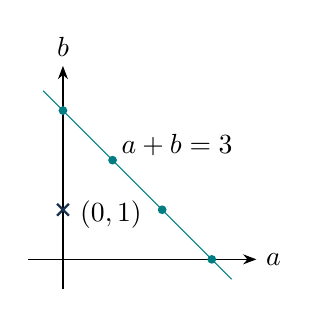
\begin{tikzpicture}[scale=.63,>=Stealth]
\draw[->] (-.7,0)--(3.9,0) node[right] {$a$};
\draw[->] (0,-.6)--(0,3.9) node[above] {$b$};
\draw[ProofTeal] (-.4,3.4)--(3.4,-.4);
\foreach \a/\b in {0/3,1/2,2/1,3/0}{\fill[ProofTeal] (\a,\b) circle(2.5pt);}
\draw[ProofNavy,thick] (-.12,.88)--(.12,1.12) (-.12,1.12)--(.12,.88);
\node[anchor=west] at (.15,.9) {$ (0,1)$};
\node at (2.3,2.3) {$a+b=3$};
\end{tikzpicture}
\end{column}
\end{columns}
\sourcecredit{Example 8.4.1}
\end{frame}

% Source: Example 8.4.2; retain the integer domain and integer inverse.
\begin{frame}{Solve for an inverse, then verify it}
Let $T:\Z^2\to\Z^2$ satisfy $T(m,n)=(m+n,m+2n)$.
If $(a,b)=T(m,n)$, subtracting the two equations gives
\[
 n=b-a,\qquad m=a-n=2a-b.
\]
Thus define $U:\Z^2\to\Z^2$ by $U(a,b)=(2a-b,b-a)$.
Both components are integers. Now check:
\[
\begin{aligned}
U(T(m,n))&=(2(m+n)-(m+2n),\ (m+2n)-(m+n))\\
         &=(m,n),\\[2pt]
T(U(a,b))&=((2a-b)+(b-a),\ (2a-b)+2(b-a))\\
         &=(a,b).
\end{aligned}
\]
$U$ is an inverse, so $T$ is bijective.
\sourcecredit{Example 8.4.2}
\end{frame}

% Source: Example 8.4.2, inverse proof. ASCII Prod and explicit composition are used.
\begin{frame}[fragile]{Lean: Function equality and coordinate equality}
\begin{lstlisting}
def T (p : Prod Int Int) : Prod Int Int :=
  (p.1 + p.2, p.1 + 2 * p.2)
def U (p : Prod Int Int) : Prod Int Int :=
  (2 * p.1 - p.2, p.2 - p.1)

example : And ((fun p => U (T p)) = id)
              ((fun p => T (U p)) = id) := by
  constructor <;> ext p <;> dsimp [T, U] <;> ring
\end{lstlisting}
\begin{itemize}
\item \texttt{Prod Int Int} is the ASCII spelling of $\Z\times\Z$.
\item \texttt{p.1} and \texttt{p.2} access the two coordinates.
\item \texttt{<;>} sends the following tactic to every generated goal.
\end{itemize}
\sourcecredit{Example 8.4.2; illustrative textbook-environment code}
\end{frame}

% Source: Example 8.4.9, p(a,b)=A(a+b)+b. Diagram is original.
\begin{frame}{Enumerating pairs of natural numbers}
\begin{block}{Theorem}
There exists a bijection $\N^2\to\N$.
\end{block}
\begin{columns}[T]
\begin{column}{.51\textwidth}
Define $A_0=0$ and $A_{s+1}=A_s+s+1$.
The first values are $0,1,3,6,10,\ldots$.
\[
 p(a,b)=A_{a+b}+b.
\]
On diagonal $a+b=s$, the second coordinate $b$ runs from $0$ through $s$.
Thus this diagonal gets the labels $A_s,\ldots,A_s+s$.
\end{column}
\begin{column}{.45\textwidth}
\centering
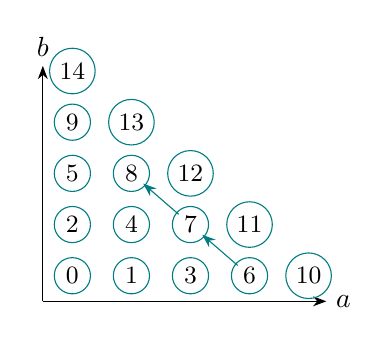
\begin{tikzpicture}[x=.75cm,y=.65cm,>=Stealth]
\draw[->] (-.5,-.5)--(4.3,-.5) node[right] {$a$};
\draw[->] (-.5,-.5)--(-.5,4.1) node[above] {$b$};
\foreach \a/\b/\lab in {0/0/0,1/0/1,0/1/2,2/0/3,1/1/4,0/2/5,3/0/6,2/1/7,1/2/8,0/3/9,4/0/10,3/1/11,2/2/12,1/3/13,0/4/14}{
  \node[draw=ProofTeal,circle,inner sep=2pt,font=\small] at (\a,\b) {\lab};}
\draw[->,ProofTeal] (2.8,.2)--(2.2,.8);
\draw[->,ProofTeal] (1.8,1.2)--(1.2,1.8);
\end{tikzpicture}
\end{column}
\end{columns}
\sourcecredit{Example 8.4.9}
\end{frame}

% Source: Example 8.4.9. This is an alternative interval proof, not a transcription
% of the book's monotonicity/intertwining Lean proof.
\begin{frame}{Why the diagonal enumeration is a bijection}
Diagonal $s$ receives exactly the integer interval
\[
 I_s=\{A_s,A_s+1,\ldots,A_s+s\}
     =\{A_s,\ldots,A_{s+1}-1\}.
\]
\textbf{Injectivity.} Different diagonals have disjoint intervals, since the
intervals are consecutive and $A_s$ strictly increases. Equal labels therefore
have the same $s$. Within that diagonal, $A_s+b$ determines $b$, and then $a=s-b$.
\medskip

\textbf{Surjectivity.} $I_0=\{0\}$ and each interval starts just after the previous one ends.
They cover $\N$: inductively, the successor of a covered number stays in its interval
or is the first number of the next interval.
If $k\in I_s$, take $b=k-A_s$ and $a=s-b$. Then $0\le b\le s$ and $p(a,b)=k$.
\sourcecredit{Example 8.4.9; alternative written proof of the same construction}
\end{frame}

% Source: Example 8.4.3; optional transfer task from Example 8.4.6.
\begin{frame}{Practice 8.4: Check that the inverse stays in the domain}
Consider $H(m,n)=(m+n,m-n)$.
\begin{enumerate}
\item Prove $H:\R^2\to\R^2$ is bijective by constructing an inverse.
\item Decide whether the same rule gives a bijection $\Z^2\to\Z^2$.
Test the target $(0,1)$.
\item Further practice: prove $(m,n)\mapsto5m+8n$ is surjective from $\Z^2$ to $\Z$.
Use $5(-3)+8(2)=1$.
\end{enumerate}
Solving equations over $\R$ does not ensure the resulting preimage has integer coordinates.
\sourcecredit{Examples 8.4.3 and 8.4.6}
\end{frame}

% Source: Newly organized solutions to Examples 8.4.3 and 8.4.6.
\begin{frame}{Practice 8.4: Solution ideas}
\begin{enumerate}
\item Over $\R$, set $K(a,b)=((a+b)/2,(a-b)/2)$. Then
\[
 K(H(m,n))=(m,n),\qquad
 H(K(a,b))=\left(\tfrac{a+b+a-b}{2},\tfrac{a+b-a+b}{2}\right)=(a,b).
\]
\item Over $\Z$, $H(m,n)=(0,1)$ would give $m+n=0$ and $m-n=1$.
Adding gives $2m=1$, impossible for an integer $m$. Hence $H$ is not surjective.
\item For any $z\in\Z$, the pair $(-3z,2z)$ is an integer preimage:
$5(-3z)+8(2z)=z$.
\end{enumerate}
\sourcecredit{Examples 8.4.3 and 8.4.6}
\end{frame}

% Source: Chapter 8 review synthesized from all four sections.
\begin{frame}{Chapter 8 review: Choose the obligation first}
\begin{center}
\begin{tabular}{p{.24\textwidth}p{.64\textwidth}}
\toprule
Goal & Useful first move\\\midrule
Injective & Assume equal outputs; recover equal inputs.\\
Not injective & Exhibit distinct inputs with equal outputs.\\
Surjective & Fix a target; construct a preimage in the domain.\\
Not surjective & Exhibit a target and rule out every preimage.\\
Bijective & Prove both properties, or verify an inverse.\\
Equal functions & Use an arbitrary input; in Lean, \texttt{ext}.\\
Equal pairs & Compare the corresponding coordinates.\\
\bottomrule
\end{tabular}
\end{center}
\textbf{Exit check.} Explain exactly why division by $2$ is harmless over $\R$
but can obstruct a claimed inverse over $\Z$.
\sourcecredit{Sections 8.1--8.4}
\end{frame}

% Source and adaptation statement for the whole chapter.
\begin{frame}{Reading and code context}
Heather Macbeth, \emph{The Mechanics of Proof}, Chapter 8:
\begin{itemize}
\item 8.1 Injectivity and surjectivity
\item 8.2 Bijectivity
\item 8.3 Composition of functions
\item 8.4 Product types
\end{itemize}
\url{https://hrmacbeth.github.io/math2001/08_Functions.html}
\medskip

These notes reorganize selected examples and supply new explanations and diagrams.
Lean listings illustrate the textbook's teaching environment, including
\texttt{addarith}, \texttt{numbers}, and \texttt{exhaust}. ASCII type names such as
\texttt{Real} and \texttt{Prod Int Int} spell out the corresponding mathematical types.
\end{frame}
\end{document}
